% TeX eps-loader file generated by stoch_simul.m (Dynare).
% 14-May-2025 09:54:31
 
\begin{figure}[H]
\centering 
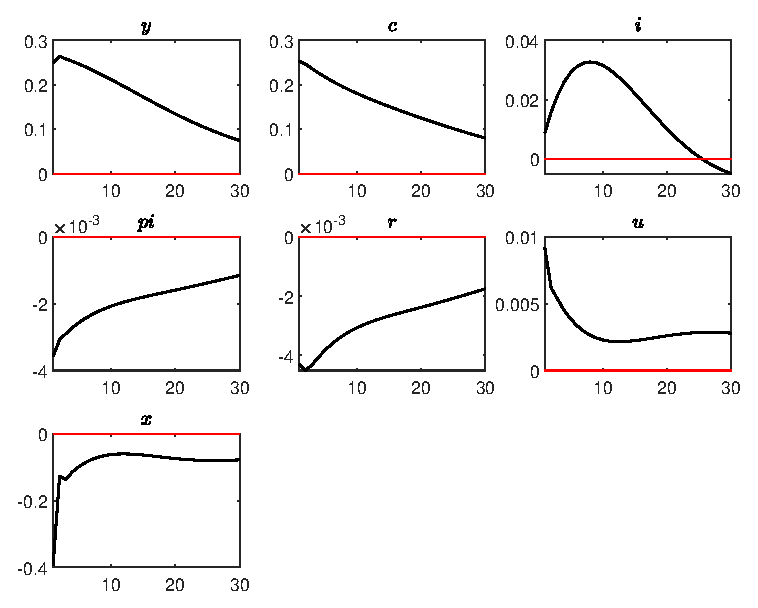
\includegraphics[width=0.80\textwidth]{unemp_argentina_baseline/graphs/unemp_argentina_baseline_IRF_eta_a}
\caption{Impulse response functions (orthogonalized shock to $eta\_a$).}
\label{Fig:IRF:eta_a}
\end{figure}
 
\begin{figure}[H]
\centering 
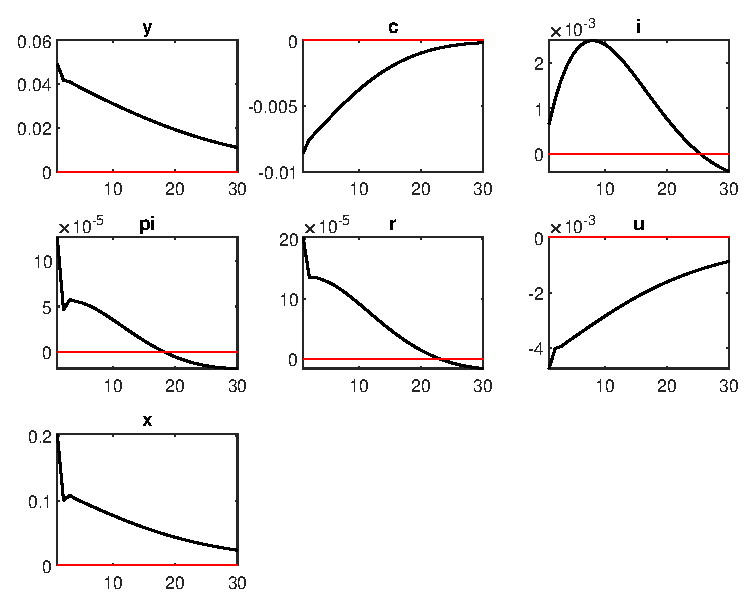
\includegraphics[width=0.80\textwidth]{unemp_argentina_baseline/graphs/unemp_argentina_baseline_IRF_eta_g}
\caption{Impulse response functions (orthogonalized shock to $eta\_g$).}
\label{Fig:IRF:eta_g}
\end{figure}
 
\begin{figure}[H]
\centering 
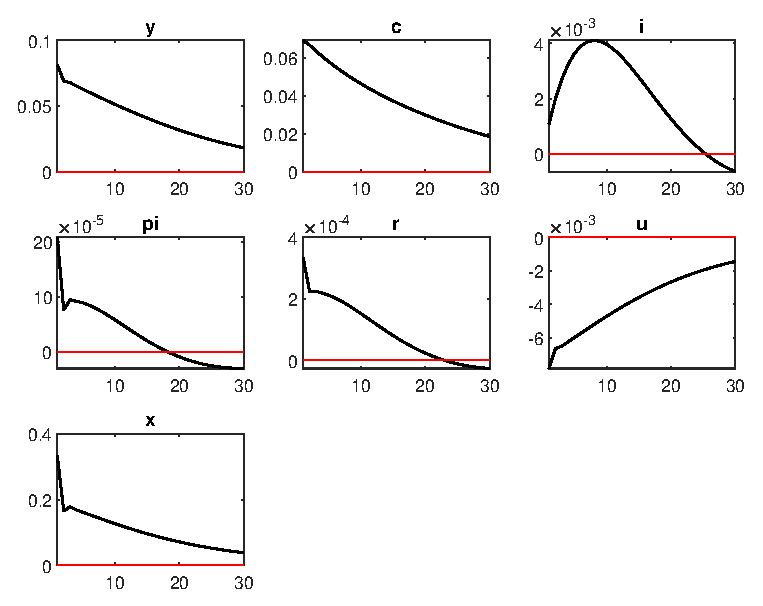
\includegraphics[width=0.80\textwidth]{unemp_argentina_baseline/graphs/unemp_argentina_baseline_IRF_eta_c}
\caption{Impulse response functions (orthogonalized shock to $eta\_c$).}
\label{Fig:IRF:eta_c}
\end{figure}
 
\begin{figure}[H]
\centering 
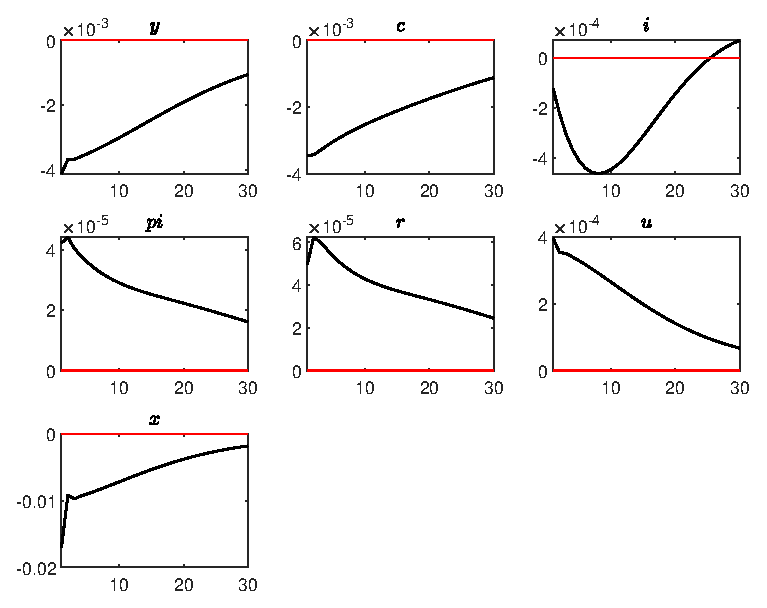
\includegraphics[width=0.80\textwidth]{unemp_argentina_baseline/graphs/unemp_argentina_baseline_IRF_eta_m}
\caption{Impulse response functions (orthogonalized shock to $eta\_m$).}
\label{Fig:IRF:eta_m}
\end{figure}
 
\begin{figure}[H]
\centering 
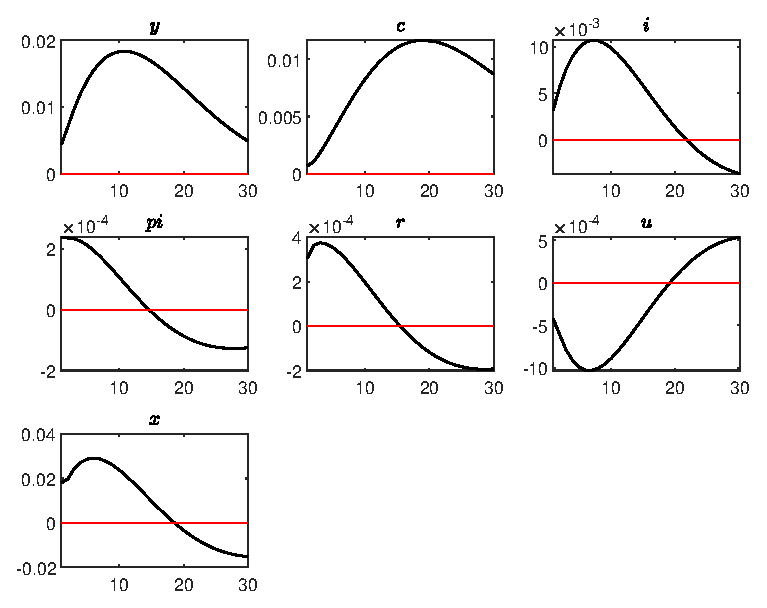
\includegraphics[width=0.80\textwidth]{unemp_argentina_baseline/graphs/unemp_argentina_baseline_IRF_eta_i}
\caption{Impulse response functions (orthogonalized shock to $eta\_i$).}
\label{Fig:IRF:eta_i}
\end{figure}
 
\begin{figure}[H]
\centering 
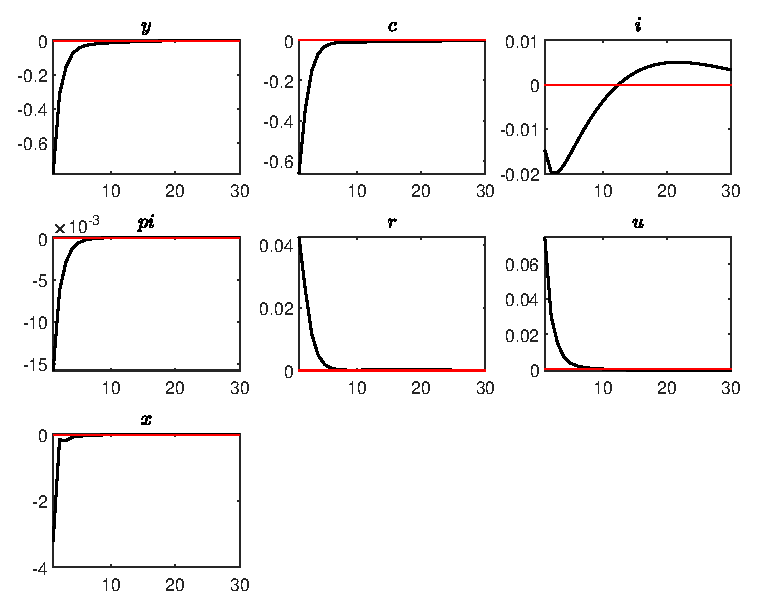
\includegraphics[width=0.80\textwidth]{unemp_argentina_baseline/graphs/unemp_argentina_baseline_IRF_eta_r}
\caption{Impulse response functions (orthogonalized shock to $eta\_r$).}
\label{Fig:IRF:eta_r}
\end{figure}
 
 
% End Of TeX file. 
